\documentclass[a4paper,12pt]{article}
\usepackage[T2A]{fontenc}
\usepackage[utf8]{inputenc}
\usepackage[russian]{babel}
\usepackage{amsmath}
\usepackage{amssymb}
\usepackage{booktabs}
\usepackage{geometry}
\usepackage{graphicx}
\usepackage{float}
\usepackage{array}
\usepackage{caption}
\geometry{margin=2.2cm}
\setlength{\parindent}{1.25cm}
\setlength{\parskip}{0.25em}

\begin{document}

\begin{center}
{\large Московский физико-технический институт}\\[0.5em]
{\large Лабораторная работа 4.7.2}\\[0.5em]
{\Large \textbf{Эффект Поккельса}}\\[1em]
Евгений Иванов, группа 5-407
\end{center}

\section*{Цель работы}
Исследовать интерференцию рассеянного света, прошедшего кристалл ниобата лития, определить двулучепреломление $n_o-n_e$, оценить полуволновое напряжение $U_{\lambda/2}$ по постоянному и переменному напряжениям и проверить выполнение условия круговой поляризации.

\section*{Оборудование и установка}
В работе использовались гелий-неоновый лазер, поляризатор, кристалл ниобата лития, матовая пластинка, экран, источник постоянного и переменного высокого напряжения, фотодиод, осциллограф и линейка. В оптической части установки лазерный луч рассеивался матовой пластинкой и проходил через кристалл, после чего на экране наблюдалась коноскопическая картина. Для исследования эффекта Поккельса без матовой пластинки за кристаллом ставились анализатор и затем фотодиод с осциллографом.

\section*{Краткая теория}
Для необыкновенной волны в одноосном кристалле показатель преломления зависит от угла $\theta$ между направлением луча и оптической осью:
\begin{equation}
\frac{1}{n_2^2}=\frac{\cos^2\theta}{n_o^2}+\frac{\sin^2\theta}{n_e^2}.
\end{equation}
Для малых углов разность фаз между обыкновенной и необыкновенной волнами после прохождения кристалла длиной $\ell$ равна
\begin{equation}
\Delta\varphi=\frac{2\pi}{\lambda}\,\ell\,(n_o-n_e)\theta^2.
\end{equation}
В случае скрещённых поляризаций радиусы тёмных колец удовлетворяют соотношению
\begin{equation}
r_m^2=\frac{\lambda}{\ell}\frac{(n_oL)^2}{n_o-n_e}\,m,
\label{eq:rings}
\end{equation}
где $L$ --- расстояние от кристалла до экрана.

При подаче напряжения на кристалл в плоскости, перпендикулярной оптической оси, возникают новые главные направления, а наведённое двулучепреломление вызывает фазовый сдвиг
\begin{equation}
\Delta\varphi=\frac{4\pi}{\lambda}\frac{\ell}{d}AU.
\end{equation}
Для скрещённых поляризаций интенсивность на выходе анализатора имеет вид
\begin{equation}
I_{\text{вых}}=I_0\sin^2\left(\frac{\pi}{2}\frac{U}{U_{\lambda/2}}\right),
\label{eq:crossed}
\end{equation}
а для параллельных поляризаций
\begin{equation}
I_{\text{вых}}=I_0\cos^2\left(\frac{\pi}{2}\frac{U}{U_{\lambda/2}}\right).
\label{eq:parallel}
\end{equation}
Полуволновое напряжение определяется формулой
\begin{equation}
U_{\lambda/2}=\frac{\lambda}{4A}\frac{d}{\ell}.
\label{eq:uhalf}
\end{equation}
При $U=U_{\lambda/2}$ фазовый сдвиг равен $\pi$, а при $U=U_{\lambda/4}=U_{\lambda/2}/2$ он равен $\pi/2$, поэтому свет на выходе кристалла становится поляризованным по кругу.

Для данной работы по учебнику использовались параметры $\lambda=0.63~\text{мкм}$, $n_o=2.29$, размеры кристалла $3\times3\times26~\text{мм}$, то есть $\ell=26~\text{мм}$ и $d=3~\text{мм}$.

\section*{Методика измерений}
Сначала при скрещённых поляризациях и установленной матовой пластинке измерялись диаметры тёмных интерференционных колец. По этим данным вычислялись радиусы $r_m$, строился график $r_m^2(m)$ и по наклону прямой с помощью формулы~\eqref{eq:rings} находилось двулучепреломление кристалла.

Далее матовая пластинка убиралась и при постоянном напряжении фиксировались характерные точки зависимости интенсивности от напряжения для скрещённых и параллельных поляризаций. Полуволновое напряжение определялось по расстоянию между соседними экстремумами. Для переменного напряжения фотодиод подключался к осциллографу, а по фигурам Лиссажу измерялось напряжение $\Delta U$, соответствующее переходу от максимума к минимуму сигнала.

\section*{Экспериментальные данные}
\subsection*{Интерференционные кольца}
Расстояние от кристалла до экрана принималось равным $L=(47.9\pm0.1)~\text{см}$. В исходной полевой записи была допущена описка в обозначении единиц, которая была исправлена при переносе данных в расчётную таблицу.

\begin{table}[H]
\centering
\caption{Измеренные диаметры и вычисленные радиусы тёмных колец}
\begin{tabular}{cccccc}
\toprule
$m$ & $d_m$, см & $\Delta d_m$, см & $r_m$, см & $\Delta r_m$, см & $r_m^2$, см$^2$ \\
\midrule
1 & 5.5 & 1.0 & 2.75 & 0.50 & 7.56 \\
2 & 8.0 & 1.0 & 4.00 & 0.50 & 16.00 \\
3 & 9.5 & 1.0 & 4.75 & 0.50 & 22.56 \\
4 & 11.5 & 1.0 & 5.75 & 0.50 & 33.06 \\
5 & 12.5 & 1.0 & 6.25 & 0.50 & 39.06 \\
\bottomrule
\end{tabular}
\end{table}

\subsection*{Характерные напряжения при постоянном напряжении}
Напряжение снималось по аналоговому вольтметру. В таблицу занесены отсчёты в делениях шкалы, а затем выполнен пересчёт в вольты при цене деления $15~\text{В}$.

\begin{table}[H]
\centering
\caption{Точки, отмеченные в ходе наблюдения зависимости интенсивности от напряжения}
\begin{tabular}{ccccccc}
\toprule
Точка & $n_{\perp}$, дел. & $U_{\perp}$, В & $\Delta U_{\perp}$, В & $n_{\parallel}$, дел. & $U_{\parallel}$, В & $\Delta U_{\parallel}$, В \\
\midrule
$U_{\lambda/2}$ & 30 & 450 & 150 & 60 & 900 & 30 \\
$U_{\lambda}$ & 60 & 900 & 30 & 85 & 1275 & 30 \\
$U_{3\lambda/2}$ & 85 & 1275 & 75 & 105 & 1575 & 30 \\
\bottomrule
\end{tabular}
\end{table}

Для состояния, близкого к четвертьволновому, в заметках был записан отсчёт $30\pm5$ делений, что после пересчёта даёт $U_{\lambda/4}\approx(450\pm75)~\text{В}$. Это значение далее используется только как качественная отметка при наблюдении круговой поляризации.

\subsection*{Осциллограф}
По фигурам Лиссажу для скрещённых поляризаций получено
\[
U_{\lambda/2}^{(\text{перем.})}=(375\pm30)\,\text{В}.
\]

\section*{Обработка результатов}
\subsection*{График $r_m^2(m)$}
Аппроксимация выполнялась прямой, проходящей через начало координат:
\[
r_m^2 = k m, \qquad k=(7.87\pm0.72)\,\text{см}^2.
\]

\begin{figure}[H]
\centering
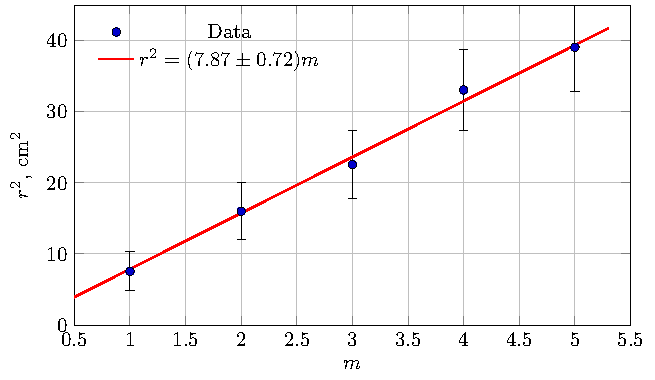
\includegraphics[width=0.8\linewidth]{rings_fit.pdf}
\caption{Зависимость $r_m^2$ от номера кольца}
\end{figure}

Тогда из формулы~\eqref{eq:rings}
\[
n_o-n_e=\frac{\lambda(n_oL)^2}{\ell k}.
\]
Подставляя $\lambda=0.63\cdot10^{-4}~\text{см}$, $n_o=2.29$, $L=47.9~\text{см}$, $\ell=2.6~\text{см}$ и найденный наклон, получаем
\[
n_o-n_e = 0.0370 \pm 0.0034.
\]

\subsection*{Полуволновое напряжение при постоянном напряжении}
При постоянном напряжении величина $U_{\lambda/2}$ определялась по расстоянию между соседними экстремумами зависимости $I_{\text{вых}}(U)$, поскольку абсолютная привязка к нулю напряжения по записям неоднозначна. Использовались четыре интервала:
\[
450\pm152.9~\text{В},\quad 375\pm80.8~\text{В},\quad 375\pm42.4~\text{В},\quad 300\pm42.4~\text{В}.
\]
Их взвешенное среднее равно
\[
U_{\lambda/2}^{(\text{пост.})} = (346\pm28)\,\text{В}.
\]

Соответствующее четвертьволновое напряжение по этой оценке должно быть
\[
U_{\lambda/4}=\frac{U_{\lambda/2}}{2}=(173\pm14)\,\text{В}.
\]
Запись $U_{\lambda/4}\approx(450\pm75)~\text{В}$ в полевых заметках этой оценке не соответствует, поэтому её можно рассматривать только как грубую визуальную отметку момента, когда поляризация казалась близкой к круговой.

\subsection*{Сравнение с измерением по фигурам Лиссажу}
Из осциллографического измерения получено
\[
U_{\lambda/2}^{(\text{перем.})}=(375\pm30)\,\text{В}.
\]
Это значение согласуется с результатом для постоянного напряжения в пределах погрешности:
\[
U_{\lambda/2}^{(\text{пост.})}=(346\pm28)\,\text{В}, \qquad
U_{\lambda/2}^{(\text{перем.})}=(375\pm30)\,\text{В}.
\]

\subsection*{Оценка изменения показателя преломления}
При $U=U_{\lambda/2}$ фазовый сдвиг равен $\pi$, поэтому из соотношения
\[
\Delta\varphi=\frac{2\pi}{\lambda}\ell\,(2\Delta n)=\pi
\]
следует
\[
\Delta n=\frac{\lambda}{4\ell}=\frac{0.63\cdot10^{-6}}{4\cdot26\cdot10^{-3}}
\approx 6.1\cdot10^{-6}.
\]
Относительное изменение показателя преломления составляет
\[
\frac{\Delta n}{n_o}\approx 2.6\cdot10^{-6}.
\]

\section*{Иллюстрации фигур Лиссажу}
На фотографиях, сделанных в работе, зафиксированы характерные фигуры Лиссажу для трёх значений напряжения при скрещённых поляризациях.

\begin{figure}[H]
\centering
\begin{minipage}[t]{0.32\linewidth}
\centering
\includegraphics[width=\linewidth]{photos/0.5.png}
\caption*{$U\approx U_{\lambda/2}$}
\end{minipage}\hfill
\begin{minipage}[t]{0.32\linewidth}
\centering
\includegraphics[width=\linewidth]{photos/1.png}
\caption*{$U\approx U_{\lambda}$}
\end{minipage}\hfill
\begin{minipage}[t]{0.32\linewidth}
\centering
\includegraphics[width=\linewidth]{photos/1.5.png}
\caption*{$U\approx U_{3\lambda/2}$}
\end{minipage}
\caption{Фигуры Лиссажу для разных напряжений}
\end{figure}

\section*{Обсуждение результатов}
График $r_m^2(m)$ близок к линейному, что соответствует формуле~\eqref{eq:rings}. Основной вклад в погрешность результата даёт довольно грубое измерение диаметров колец с одинаковой ошибкой порядка $1~\text{см}$. Дополнительная неопределённость связана с тем, что при переносе полевых записей пришлось исправить описку в единицах для расстояния $L$.

Оценки $U_{\lambda/2}$ по постоянному и переменному напряжениям хорошо согласуются между собой. Отсчёт для режима, близкого к $U_{\lambda/4}$, носил скорее качественный характер, так как этот момент определялся по визуальному наблюдению изменения поляризации при вращении анализатора.

\section*{Заключение}
По измеренным радиусам интерференционных колец найдено двулучепреломление кристалла ниобата лития:
\[
n_o-n_e = 0.0370 \pm 0.0034.
\]
Полуволновое напряжение, определённое по постоянному напряжению, равно
\[
U_{\lambda/2}^{(\text{пост.})}=(346\pm28)\,\text{В},
\]
а по фигурам Лиссажу при переменном напряжении
\[
U_{\lambda/2}^{(\text{перем.})}=(375\pm30)\,\text{В}.
\]
Обе оценки согласуются в пределах погрешности. При таком напряжении изменение показателя преломления имеет порядок $10^{-6}$.

\begin{thebibliography}{9}
\bibitem{optics-lab}
Лабораторный практикум по общей физике. В 3 т. Т. 2: Оптика. Раздел 4.7.2 ``Эффект Поккельса''.
\end{thebibliography}

\end{document}
